% Fig. 1: single-column overview of the method: the spiking command layer in the control loop (top) and its
% three-stage training with evolution strategies (bottom).
% Build:  cd figures/tikz && pdflatex overview_diagram.tex   (needs flapsim_render.jpg in the same folder)
\documentclass[border=1pt]{standalone}
\pdfsuppressptexinfo=-1  % do not copy the info dictionaries (author names) of included PDFs
\pdfinfo{/Author () /Title ()}
\usepackage{newtxtext,newtxmath}
\usepackage{tikz}
\usetikzlibrary{arrows.meta,calc,positioning}
\definecolor{snn}{HTML}{1764D6}
\definecolor{snnedge}{HTML}{0B3D8C}
\definecolor{snnfill}{HTML}{EAF2FD}
\definecolor{snnlight}{HTML}{86B6EF}
\definecolor{cls}{HTML}{4A4844}
\definecolor{ink2}{HTML}{52514E}
\definecolor{muted}{HTML}{898781}
\definecolor{grid}{HTML}{D9D7D0}
\definecolor{ok}{HTML}{1E8E3E}
\begin{document}
\begin{tikzpicture}[
    >={Stealth[length=5pt,width=4pt]},
    tiny/.style={font=\fontsize{7.4pt}{8.0pt}\selectfont, text=ink2, inner sep=1pt},
    lbl/.style={font=\fontsize{7.6pt}{8.4pt}\selectfont, text=black, inner sep=1pt},
    tag/.style={font=\fontsize{7.8pt}{8.8pt}\selectfont\bfseries, text=black, inner sep=1pt},
    bg/.style={fill=white, inner sep=1.2pt},
    neuron/.style={circle, draw=snnedge, line width=.7pt, fill=white, minimum size=2.3mm, inner sep=0},
    flow/.style={->, line width=1.1pt, draw=ink2},
  ]
  % ================= control loop =================
  % environment
  \node[inner sep=0] (sim) at (1.2,3.75) {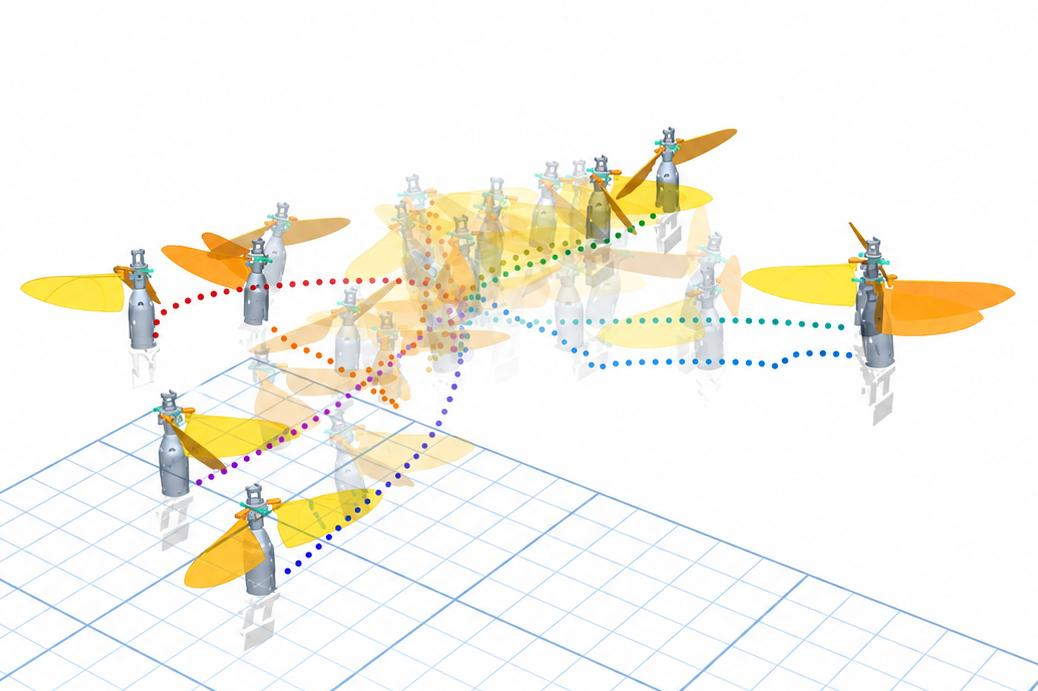
\includegraphics[width=2.3cm]{flapsim_render.jpg}};
  \node[tag, below=.5mm of sim] {FlapSim};

  % spiking command layer
  \fill[snnfill, rounded corners=4pt] (2.88,1.98) rectangle (6.55,5.42);
  \draw[snnedge, line width=1.0pt, rounded corners=4pt] (2.88,1.98) rectangle (6.55,5.42);
  \node[tag, text=snnedge, anchor=south] at (4.72,5.47) {spiking command layer (2{,}564 params)};

  % inputs with delay taps
  \foreach \i/\y in {1/4.55, 2/4.15, 3/3.75, 4/3.35, 5/2.95} {
    \node[circle, fill=muted, minimum size=1.6mm, inner sep=0] (in\i) at (3.45,\y) {};
    \foreach \k in {1,2,3} \fill[grid!80!black] ($(in\i)+(-.13-.09*\k,-.03)$) rectangle ++(.06,.06);
  }
  % 8 leaky integrate-and-fire neurons with spike trains
  \foreach \j/\y in {1/4.68, 2/4.39, 3/4.10, 4/3.81, 5/3.52, 6/3.23, 7/2.94, 8/2.65} {
    \node[neuron] (h\j) at (4.45,\y) {};
  }
  \foreach \i in {1,...,5} \foreach \j in {1,...,8} \draw[snnlight, line width=.35pt, opacity=.6] (in\i) -- (h\j);
  \foreach \j/\ts in {1/{.05,.21,.30}, 2/{.12,.27}, 3/{.02,.15,.33}, 4/{.20}, 5/{.08,.25}, 6/{.01,.14,.29}, 7/{.17,.31}, 8/{.04,.22}} {
    \foreach \t in \ts \draw[snnedge, line width=.7pt] ($(h\j)+(.2+\t,-.07)$) -- ++(0,.14);
  }
  % outputs: two spiking neurons, two graded units
  \node[neuron, fill=snn] (o1) at (6.0,4.30) {};
  \node[neuron, fill=snn] (o2) at (6.0,3.95) {};
  \node[draw=snnedge, line width=.7pt, fill=snnlight, minimum size=2.1mm, inner sep=0] (o3) at (6.0,3.30) {};
  \node[draw=snnedge, line width=.7pt, fill=snnlight, minimum size=2.1mm, inner sep=0] (o4) at (6.0,2.95) {};
  \foreach \j in {1,...,8} \foreach \o in {o1,o2,o3,o4} \draw[snnlight, line width=.35pt, opacity=.6] ($(h\j)+(.62,0)$) -- (\o);
  \node[tiny, align=center] at (3.48,2.27) {25 inputs\\[-1pt]$\times$11 taps};
  \node[tiny, align=center] at (4.66,2.27) {8 LIF\\[-1pt]neurons};
  \node[tiny, align=center] at (5.9,2.27) {2 spiking\\[-1pt]+ 2 graded};

  % actions (all labels clear of the lines)
  \draw[snnedge, line width=1.1pt] (6.85,4.0) -- (7.25,4.0) -- (7.25,4.42) -- (7.6,4.42) -- (7.6,4.0) -- (8.45,4.0);
  \node[lbl, anchor=south] at (7.43,4.55) {motor pulse};
  \node[tiny, anchor=north, align=center] at (8.0,3.92) {at a chosen\\[-1pt]wingbeat phase};
  \node[lbl, anchor=west, align=left] at (6.92,2.98) {set-points $\alpha^\ast\!,\beta^\ast$\\[-1pt]{\fontsize{7.4pt}{8.0pt}\selectfont\color{ink2} PID $\rightarrow$ gimbal}};
  \draw[flow] (o2.east) ++(.06,0) -- (6.80,4.0);
  \draw[flow] (o3.east) ++(.06,0) -- (6.86,3.14);

  % loop closure
  \draw[flow] (sim.east) ++(0,-.05) -- (2.86,3.7);
  \node[tiny, anchor=south] at (2.6,3.78) {IMU};
  \draw[flow, rounded corners=3pt] (8.62,2.75) -- (8.62,1.70) -- (1.2,1.70) -- (1.2,2.75);
  \node[tiny, anchor=north] at (3.55,1.62) {motor speed $\omega$, gimbal $\alpha,\beta$};

  % ================= training with evolution strategies =================
  \node[tag, anchor=west] at (0.05,1.30) {training};
  % stage 1: imitation of the classical controller
  \draw[cls, line width=1.0pt] plot[smooth, domain=0:1.9, samples=30] (\x+0.2, {0.65+0.28*sin(220*\x)});
  \draw[snn, line width=1.0pt, dashed] plot[smooth, domain=0:1.9, samples=30] (\x+0.2, {0.62+0.25*sin(220*\x-14)});
  \node[lbl, align=center] at (1.15,0.08) {1\enspace imitation (BPTT)};
  % stage 2: OpenAI-ES around the centre, on a shaded fitness landscape (darker = better score)
  \shade[inner color=snn!45, outer color=white] (4.55,.78) ellipse (1.05 and .48);
  \foreach \r in {.33,.66,1.0} \draw[snnlight!70!snnedge, line width=.55pt, opacity=.8] (4.55,.78) ellipse ({1.05*\r} and {.48*\r});
  \coordinate (th) at (3.95,.62);
  \foreach \a/\c in {20/70,75/45,130/30,200/25} {
    \fill[snn!\c!white, draw=snnedge, line width=.3pt] ($(th)+(\a:.28)$) circle (.05);
    \fill[snn!\c!white, draw=snnedge, line width=.3pt] ($(th)+(\a+180:.28)$) circle (.05);
    \draw[snnedge!60, line width=.45pt] ($(th)+(\a:.23)$) -- ($(th)+(\a+180:.23)$);
  }
  \fill[snnedge] (th) circle (.075);
  \draw[->, snnedge, line width=1.1pt] (th) -- (4.45,.77);
  \node[tiny, text=snnedge, anchor=east] at ($(th)+(-.33,.07)$) {$\theta$};
  \node[lbl, align=center] at (4.55,0.08) {2\enspace OpenAI-ES, antithetic pairs};
  % stage 3: selection and freezing (bold outline, green check)
  \draw[snnedge, line width=1.6pt, rounded corners=3pt, fill=white] (6.88,-.12) rectangle (8.55,1.15);
  \draw[ok, line width=1.3pt, fill=ok!8] (7.71,.70) circle (.3);
  \draw[ok, line width=2.2pt, line cap=round, line join=round] (7.55,.71) -- (7.67,.57) -- (7.88,.88);
  \node[lbl, align=center] at (7.71,0.1) {\textbf{3}\enspace select, freeze};
  % flow between stages and into the network
  \draw[flow] (2.22,.68) -- (2.95,.68);
  \draw[flow] (5.65,.68) -- (6.84,.68);
  \draw[flow, dashed, snnedge] (7.71,1.17) -- (7.71,1.55) -| (6.3,1.96);
  \node[tiny, text=snnedge, anchor=west] at (7.78,1.36) {frozen weights};
\end{tikzpicture}
\end{document}
